\documentclass[a4paper,11pt]{scrreprt}
\usepackage{tikz}

\newcommand*{\code}[1]{\texttt{#1}}
\newcommand*{\defi}[1]{\textbf{#1}}

\title{Technical supplement to the COVID19 report}
\author{Hugh Parsonage}

\providecommand{\crema}{\textsc{crema}}


\begin{document}

\addchap{Overview}
Our model, \crema, is a dynamic microsimulation model of Australia. 

\subsection{Static data}
The model runs on a static data table, each row a person in Australia, 
which identifies each person's

\begin{enumerate}
	\item state and SA2,
	\item age
	\item household
	\item school,
	\item labour force status,
\end{enumerate}

For performance reasons, data is cached before being passed to the dynamic model.
Obviously, the cache includes the static data. Other features of each person is 
also cached (or ``generated at cache time''). Cache time variables include:

\begin{description}
\item[\code{SupermarketTypical}] If an individual's SA2 contains zero supermarkets, 
a value of zero. 
For implementation convenience,%
	\footnote{By \defi{implementation convenience}, I mean that the choice was not made 
	on the basis of research, because it was necessary to do so and was not considered 
	sufficiently important to make more than an arbitrary decision. In this case,
	the choice of 8 was made to avoid stack overflow.}
If the individual's SA2 contains more than eight supermarket we 
exclude all but eight supermarkets. We then assign to each person a random integer
from 1 to \(N_S = {}\) the number of supermarkets in each SA2 to represent the 
`typical' supermarket a person visits.
\end{description}

For technical reasons, we shorten variables so that they are a sequence. 

\subsection{Assignment of individuals to workplaces}
While we are confident about the distribution of labour force status among
the population we assign in the static data, we do not know how large each 
worker's workplace is. To model this, for each destination zone we construct
a sequence of geometrically distributed random variables with parameters 
\(1/\beta = 1/15\). 

\begin{figure}[!htbp]
\caption{The geometric distribution with mean 15 over the range [0, 50]}\label{fig:geom-distr}
\makebox[\textwidth]{
	% Created by tikzDevice version 0.12.3 on 2020-05-31 18:14:11
% !TEX encoding = UTF-8 Unicode
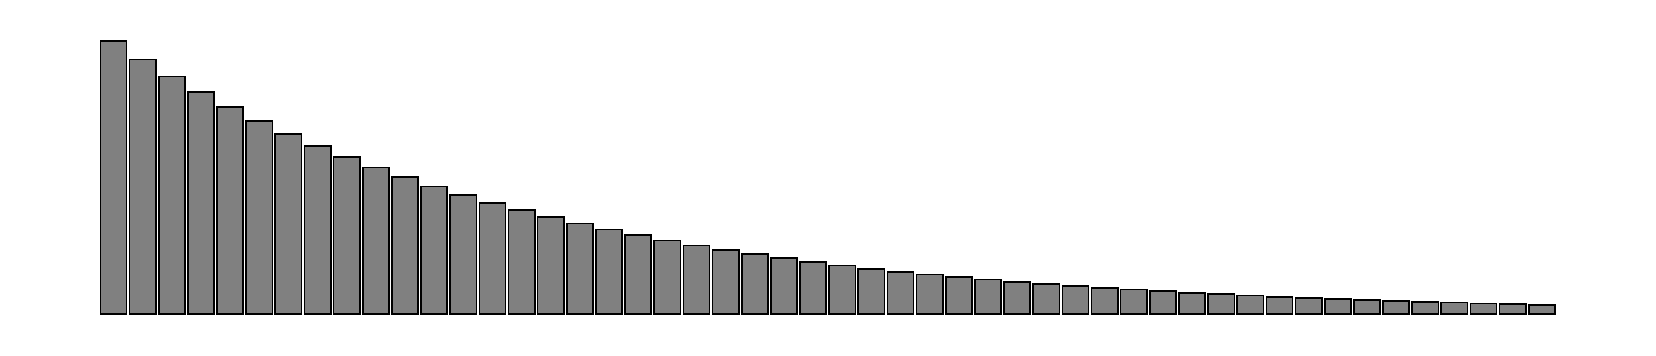
\begin{tikzpicture}[x=1pt,y=1pt]
\definecolor{fillColor}{RGB}{255,255,255}
\path[use as bounding box,fill=fillColor,fill opacity=0.00] (0,0) rectangle (578.16,108.41);
\begin{scope}
\path[clip] (  0.00,  0.00) rectangle (578.16,108.41);
\definecolor{drawColor}{RGB}{0,0,0}
\definecolor{fillColor}{RGB}{128,128,128}

\path[draw=drawColor,line width= 0.6pt,line cap=rect,fill=fillColor] ( 26.28,  4.93) rectangle ( 35.76,103.48);

\path[draw=drawColor,line width= 0.6pt,line cap=rect,fill=fillColor] ( 36.81,  4.93) rectangle ( 46.29, 96.91);

\path[draw=drawColor,line width= 0.6pt,line cap=rect,fill=fillColor] ( 47.35,  4.93) rectangle ( 56.83, 90.78);

\path[draw=drawColor,line width= 0.6pt,line cap=rect,fill=fillColor] ( 57.88,  4.93) rectangle ( 67.36, 85.05);

\path[draw=drawColor,line width= 0.6pt,line cap=rect,fill=fillColor] ( 68.41,  4.93) rectangle ( 77.89, 79.71);

\path[draw=drawColor,line width= 0.6pt,line cap=rect,fill=fillColor] ( 78.95,  4.93) rectangle ( 88.43, 74.73);

\path[draw=drawColor,line width= 0.6pt,line cap=rect,fill=fillColor] ( 89.48,  4.93) rectangle ( 98.96, 70.07);

\path[draw=drawColor,line width= 0.6pt,line cap=rect,fill=fillColor] (100.01,  4.93) rectangle (109.49, 65.73);

\path[draw=drawColor,line width= 0.6pt,line cap=rect,fill=fillColor] (110.54,  4.93) rectangle (120.02, 61.68);

\path[draw=drawColor,line width= 0.6pt,line cap=rect,fill=fillColor] (121.08,  4.93) rectangle (130.56, 57.89);

\path[draw=drawColor,line width= 0.6pt,line cap=rect,fill=fillColor] (131.61,  4.93) rectangle (141.09, 54.36);

\path[draw=drawColor,line width= 0.6pt,line cap=rect,fill=fillColor] (142.14,  4.93) rectangle (151.62, 51.07);

\path[draw=drawColor,line width= 0.6pt,line cap=rect,fill=fillColor] (152.68,  4.93) rectangle (162.16, 47.99);

\path[draw=drawColor,line width= 0.6pt,line cap=rect,fill=fillColor] (163.21,  4.93) rectangle (172.69, 45.12);

\path[draw=drawColor,line width= 0.6pt,line cap=rect,fill=fillColor] (173.74,  4.93) rectangle (183.22, 42.44);

\path[draw=drawColor,line width= 0.6pt,line cap=rect,fill=fillColor] (184.28,  4.93) rectangle (193.76, 39.94);

\path[draw=drawColor,line width= 0.6pt,line cap=rect,fill=fillColor] (194.81,  4.93) rectangle (204.29, 37.60);

\path[draw=drawColor,line width= 0.6pt,line cap=rect,fill=fillColor] (205.34,  4.93) rectangle (214.82, 35.43);

\path[draw=drawColor,line width= 0.6pt,line cap=rect,fill=fillColor] (215.88,  4.93) rectangle (225.35, 33.39);

\path[draw=drawColor,line width= 0.6pt,line cap=rect,fill=fillColor] (226.41,  4.93) rectangle (235.89, 31.50);

\path[draw=drawColor,line width= 0.6pt,line cap=rect,fill=fillColor] (236.94,  4.93) rectangle (246.42, 29.72);

\path[draw=drawColor,line width= 0.6pt,line cap=rect,fill=fillColor] (247.47,  4.93) rectangle (256.95, 28.07);

\path[draw=drawColor,line width= 0.6pt,line cap=rect,fill=fillColor] (258.01,  4.93) rectangle (267.49, 26.53);

\path[draw=drawColor,line width= 0.6pt,line cap=rect,fill=fillColor] (268.54,  4.93) rectangle (278.02, 25.09);

\path[draw=drawColor,line width= 0.6pt,line cap=rect,fill=fillColor] (279.07,  4.93) rectangle (288.55, 23.74);

\path[draw=drawColor,line width= 0.6pt,line cap=rect,fill=fillColor] (289.61,  4.93) rectangle (299.09, 22.49);

\path[draw=drawColor,line width= 0.6pt,line cap=rect,fill=fillColor] (300.14,  4.93) rectangle (309.62, 21.32);

\path[draw=drawColor,line width= 0.6pt,line cap=rect,fill=fillColor] (310.67,  4.93) rectangle (320.15, 20.23);

\path[draw=drawColor,line width= 0.6pt,line cap=rect,fill=fillColor] (321.21,  4.93) rectangle (330.69, 19.21);

\path[draw=drawColor,line width= 0.6pt,line cap=rect,fill=fillColor] (331.74,  4.93) rectangle (341.22, 18.25);

\path[draw=drawColor,line width= 0.6pt,line cap=rect,fill=fillColor] (342.27,  4.93) rectangle (351.75, 17.37);

\path[draw=drawColor,line width= 0.6pt,line cap=rect,fill=fillColor] (352.81,  4.93) rectangle (362.28, 16.54);

\path[draw=drawColor,line width= 0.6pt,line cap=rect,fill=fillColor] (363.34,  4.93) rectangle (372.82, 15.76);

\path[draw=drawColor,line width= 0.6pt,line cap=rect,fill=fillColor] (373.87,  4.93) rectangle (383.35, 15.04);

\path[draw=drawColor,line width= 0.6pt,line cap=rect,fill=fillColor] (384.40,  4.93) rectangle (393.88, 14.37);

\path[draw=drawColor,line width= 0.6pt,line cap=rect,fill=fillColor] (394.94,  4.93) rectangle (404.42, 13.74);

\path[draw=drawColor,line width= 0.6pt,line cap=rect,fill=fillColor] (405.47,  4.93) rectangle (414.95, 13.15);

\path[draw=drawColor,line width= 0.6pt,line cap=rect,fill=fillColor] (416.00,  4.93) rectangle (425.48, 12.60);

\path[draw=drawColor,line width= 0.6pt,line cap=rect,fill=fillColor] (426.54,  4.93) rectangle (436.02, 12.09);

\path[draw=drawColor,line width= 0.6pt,line cap=rect,fill=fillColor] (437.07,  4.93) rectangle (446.55, 11.61);

\path[draw=drawColor,line width= 0.6pt,line cap=rect,fill=fillColor] (447.60,  4.93) rectangle (457.08, 11.17);

\path[draw=drawColor,line width= 0.6pt,line cap=rect,fill=fillColor] (458.14,  4.93) rectangle (467.62, 10.75);

\path[draw=drawColor,line width= 0.6pt,line cap=rect,fill=fillColor] (468.67,  4.93) rectangle (478.15, 10.36);

\path[draw=drawColor,line width= 0.6pt,line cap=rect,fill=fillColor] (479.20,  4.93) rectangle (488.68, 10.00);

\path[draw=drawColor,line width= 0.6pt,line cap=rect,fill=fillColor] (489.73,  4.93) rectangle (499.21,  9.66);

\path[draw=drawColor,line width= 0.6pt,line cap=rect,fill=fillColor] (500.27,  4.93) rectangle (509.75,  9.35);

\path[draw=drawColor,line width= 0.6pt,line cap=rect,fill=fillColor] (510.80,  4.93) rectangle (520.28,  9.05);

\path[draw=drawColor,line width= 0.6pt,line cap=rect,fill=fillColor] (521.33,  4.93) rectangle (530.81,  8.78);

\path[draw=drawColor,line width= 0.6pt,line cap=rect,fill=fillColor] (531.87,  4.93) rectangle (541.35,  8.52);

\path[draw=drawColor,line width= 0.6pt,line cap=rect,fill=fillColor] (542.40,  4.93) rectangle (551.88,  8.28);
\end{scope}
\end{tikzpicture}

}
\end{figure}

The number of random variables to generate is determined algorithmically: if the next random variable
would overflow into the next DZN, we fill the rest of the sequences with 2, which has the useful 
side-effect of inflating the number of partnerships to a number consistent with observation.
With this sequence we obtain, for each working person, a group of workers associated with each person 
and the size of their workplace.








\end{document}




